\usepackage[utf8]{inputenc}
\usepackage{slovak}
\usepackage{tikz}
\usetikzlibrary{arrows,positioning}
\usetheme{Warsaw}
\bibliographystyle{apalike}
\title{Biologicky motivované \\výpočtové modely}
\author{Michal Kováč}
\institute{FMFI UK}
\date{24.6.2013}
\begin{document}

\begin{frame}[t]
\titlepage
\end{frame}
\note{Vážená komisia, \dots, chcel by som vám prezentovať moje pokroky v dizertačnej práci.}

\section*{Outline}
\begin{frame}
\tableofcontents
\end{frame}
\note{Prezentáciu začnem prehľadom existujúcich modelov, ktoré sú inšpirované biológiou.
Potom budem hovoriť o P systémoch, pretože im som sa najviac venoval.
Existuje množstvo variantov, o ktorých niečo poviem v ďalšej časti.
Prezentáciu zavŕšim predostretím plánov na dizertačnú prácu.}

\section{Prehľad problematiky} % (fold)
\label{sec:prehlad_problematiky}

\subsection{Prehľad modelov} % (fold)
\label{sub:prehlad_modelov}

\begin{frame}[t]\frametitle{Biologicky motivované \\výpočtové modely}
Modely vznikajú s dvoma účelmi:
\begin{itemize}
  \item simulácia biologických javov
  \item zdokonalenie informatických riešení
\end{itemize}
\end{frame}
\note{Tieto modely majú dvojaké uplatnenie.
Jednak v rámci biológie môžu slúžiť ako reálne modely správania sa živých systémov, na ktorých si možnosťami simulácie či verifikácie môžeme overovať správnosť nášho chápania ich biologickej činnosti, robiť virtuálne biologické experimenty.

Na druhej strane môžu slúžiť ako nové inšpiratívne výpočtové modely otvárajúce rad teoretických informatických otázok (napr. výpočtová sila) alebo ako modely na popis aj iných ako biologických systémov.}

\begin{frame}[t]\frametitle{Biologicky motivované \\výpočtové modely}
\begin{itemize}
  \item Neurónové siete (od 1943)
  \item Celulárne automaty (od 1948)
  \item Evolučné algoritmy (od 1954)
  \item L systémy (od 1968)
  \item P systémy (od 1998) \cite{Paun98}
  \item Calculi of Looping Sequences (od 2007)
  \item Reaction systems (od 2007)
  \item \dots
\end{itemize}
\end{frame}
\note{Dlho skúmané modely ako neurónové siete, celulárne automaty, evolučné algoritmy, či L systémy, si už našli svoje uplatnenie v praxi, kým membránové systémy sú ešte len v začiatkoch svojho vývoja.}

% subsection prehlad_modelov (end)

\subsection{P systémy} % (fold)
\label{sub:p_systemy}

\begin{frame}[t]\frametitle{Membránová štruktúra}
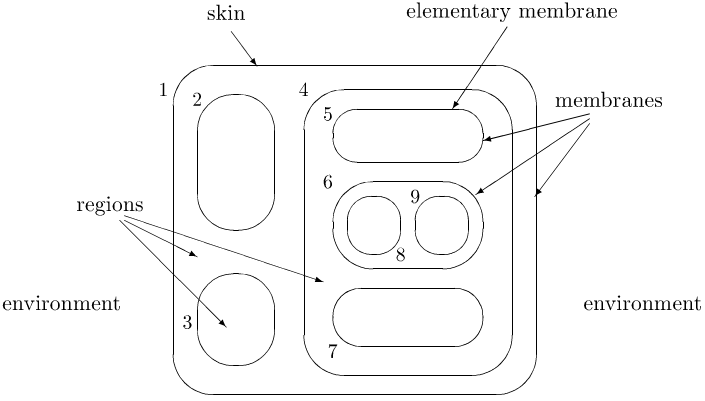
\includegraphics[width=0.7\textwidth]{membrane_structure.png}
\hfill
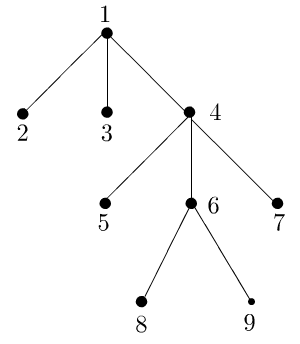
\includegraphics[width=0.3\textwidth]{membrane_tree.png}

\end{frame}
\note{Membránové systémy sú inšpirované bunkami. Základom je preto membránová štruktúra, ktorá pozostáva z regiónov, ktoré sú oddelené membránami. Tvorí to hierarchickú štruktúru, ktorá sa dá zobraziť ako strom.}

\begin{frame}[t]\frametitle{Obsah membrány}
\begin{itemize}
  \item multimnožina objektov
  \begin{itemize}
    \item $a\ |\ b\ |\ b$
  \end{itemize}
  \item prepisovacie pravidlá
  \begin{itemize}
    \item $a\ |\ b\ |\ b\rightarrow a\ |\ a_{out}\ |\ b_{in_{6}}$
    \item $b \rightarrow a\ |\ \delta$
  \end{itemize}
\end{itemize}
\end{frame}
\note{V každej membráne je multimnožina objektov. Objekty predstavujú molekuly, alebo chemické zlúčeniny.

Každá membrána má aj množinu prepisovacích pravidiel. Ľavá aj pravá strana pravidla pozostáva z multimnožiny objektov, pričom ľavá strana nesmie byť prázdna.

Posielanie objektov cez membránu sa uskutočňuje tak, že na pravej strane môžu mať objekty špecifikované, či ostanú v aktuálnom regióne, alebo sa pošlú cez membránu von, alebo dnu cez konkrétnu membránu.

Pravidlo môže obsahovať špeciálny symbol delta. Po aplikácii takéhoto pravidla sa membrána rozpustí, jej pravidlá zaniknú, a objekty a prípadne membrány sa z vnútra vylejú von.
}

\begin{frame}[t]\frametitle{P systém}

P systém definujeme ako $\Pi = (V, \mu, w_1, w_2,\dots , w_m, R_1, R_2, \dots , R_m)$, kde:
\begin{itemize}
  \item $V$ je abeceda objektov
  \item $\mu$ je membránová štruktúra
  \item $w_1, w_2, \dots w_m$ sú počiatočné multimnožiny v membránach $1\dots m$, $w_i\subseteq \mathbb{N}^V$
  \item $R_1, R_2, \dots , R_m$ sú množiny prepisovacích pravidiel v membránach $1\dots m$, pričom $$R_i\subseteq(\mathbb{N}^V\setminus 0^V)\times\mathbb{N}^{V\times(\{here,out\}\cup\{in_1,\dots in_m\})}$$.
\end{itemize}

\end{frame}
\note{P systém sa definuje ako konštrukt pozostávajúci z abecedy objektov, membránovej štruktúry, počiatočnej multimnožiny objektov a prepisovacích pravidiel}

\begin{frame}[t]\frametitle{Konfigurácia a krok výpočtu}
\begin{itemize}
  \item konfigurácia = membránová štruktúra + obsahy membrán
  \item krok výpočtu: maximálny paralelizmus
\end{itemize}
\tikzstyle{mybox} = [draw=black,very thick, rectangle, rounded corners, inner sep=10pt]
\begin{tikzpicture}
  \onslide<2->{
    \node [mybox] (box){%
      \begin{minipage}{0.50\textwidth}
        \vspace{0pt}
        \begin{align}
          \tag{$r_1$}a\ |\ b\ |\ b&\rightarrow c\\
          \tag{$r_2$}b &\rightarrow c\ |\ c
        \end{align}
        $a\ |\ a\ |\ b\ |\ b$
      \end{minipage}
    };
  }
  \onslide<3->{
    \node [mybox,below=3cm of box.west,anchor=west] (box2) {$a\ |\ c$};
    \path[-triangle 45] (box) edge [left] node {$r_1$} (box2);
  }
  \onslide<4->{
    \node [mybox,below=3cm of box.east,anchor=east] (box3){$a\ |\ a\ |\ c\ |\ c\ |\ c\ |\ c$};
    \path[-triangle 45] (box) edge [right] node {$2*r_2$} (box3);
  }
\end{tikzpicture}
\end{frame}
\note{Konfigurácia P systému v sebe zahŕňa membránovú štruktúru a obsahy jednotlivých membrán. P systém má globálny časovač, v každom kroku, každá membrána aplikuje maximálnu multimnožinu pravidiel.

V tomto príklade máme dve jednoduché pravidlá a multimnožinu aabb. Ak sa použije prvé pravidlo, žiadne ďalšie sa už v tomto kroku použiť nemôže, preto je to maximálna multimnožina.

Ak sa použije druhé pravidlo, musí sa použiť dvakrát, aby to bola maximálna multimnožina.

V tomto príklade sú teda dve maximálne multimnožiny pravidiel. O ďalšej konfigurácii sa rozhodne nedeterministicky.
}

\begin{frame}[t]\frametitle{Jazyk}
\begin{itemize}
  \item výsledok výpočtu je multimnožina objektov, ktorá:
  \begin{itemize}
    \item počas výpočtu prešla cez vonkajšiu membránu
    \item na konci ostane v špecifickej membráne
  \end{itemize}
  \item generatívny vs akceptačný mód
  \item Parikhovo zobrazenie: PsRE
\end{itemize}
\end{frame}
\note{Ak je postupnosť krokov výpočtu konečná, výpočet je úspešný a výsledok výpočtu je multimnožina objektov, ktorá prešla cez vonkajšiu membránu. Podobne by sa dal definovať aj ako multimnožina objektov, ktorá ostane v špecifickej membráne.

V akceptačnom móde sa do špecifickej membrány vloží multimnožina objektov, pričom ostatné membrány sú prázdne. Ak výpočet zastaví, pôvodná multimnožina patrí do jazyka, inak nepatrí.
}
\newpage
\note{Pre vačšinu známych modelov sú generatívny aj akceptačný mód rovnako silné, u P systémoch to nie je vždy tak, preto sa oplatí skúmať obidva módy.

Všetky možné úspešné výpočty definujú jazyk nad multimnožinami. Z hľadiska výpočtovej sily sa triedy týchto jazykov porovnávajú s Parikhovým zobrazením známych tried jazykov. P systémom zodpovedá trieda jazykov PsRE, čo je Parikov obraz triedy rekurzívne vyčísliteľných jazykov. Voláme ich univerzálne, lebo podľa Turingovej tézy nimi vieme simulovať akýkoľvek iný model, ktorý je algoritmicky simulovateľný.
}

% subsection p_systemy (end)

\subsection{Varianty} % (fold)
\label{sub:varianty}

\begin{frame}[t]\frametitle{Varianty objektov}
\begin{itemize}
  \item worm objects \cite{Mate02}
  \begin{itemize}
  \item namiesto multimnožín objektov sú v membránach multimnožiny stringov ($\mathbb{N}^{V^*}$)
    \item inšpirované DNA
  \end{itemize}
\end{itemize}
\end{frame}
\note{Aby sme mohli definovať priamo jazyky nad stringami, Mate navrhol variant P systems with worm objects. V membránach sú rovno multimnožiny stringov, čo je inšpirované reťazcami DNA. Takto dostal tiež univerzálny model.}

\begin{frame}[t]\frametitle{Varianty pravidiel}
\begin{itemize}
  \item kontextové (PsRE)
  \item kooperatívne (PsRE) \cite{Paun98}
  \item katalytické
  \begin{itemize}
    \item s 2 katalyzátormi (PsRE) \cite{Freund2005TwoCatalysts}
    \item s 1 katalyzátorom (otvorený problem)
    \item s 1 katalyzátorom a inhibítormi (PsRE) \cite{Ionescu:jucs_10_5:on_p_systems_with}
  \end{itemize}
  \item bezkontextové (PsCF) \cite{Sburlan05dragos}
  \item bezkontextové s inhibítormi (PsET0L) \cite{Ionescu:jucs_10_5:on_p_systems_with}
\end{itemize}
\end{frame}
\note{Pôvodná definícia definovala kontextové pravidlá. Ak by sme ľavú stranu obmedzili, že v nej môžu byť maximálne 2 objekty, sú to kooperatívne pravidlá. O nich Paun v pôvodnom článku ukázal, že sú tiež univerzálne.

Katalyzátory sa definujú ako podmnožina objektov. Keď sa katalyzátor nachádza na ľavej strane pravidla, musí sa aj na pravej strane. OKrem katalyzátorov sa na ľavej strane nachádza práve jeden objekt, ktorý nie je katalyzátor.
Séria článkov skúmala, koľko minimálne katalyzátorov treba na univerzálnosť. Až v roku 2005 Freund ukázal, že stačia 2 a nastolil otvorený problém, ako je to s 1 katalyzátorom. Jediné, na čo sa prišlo, je, že keď sa použijú navyše inhibítory, tak je to univerzálne.
}
\newpage
\note{
Bezkontextové pravidlá majú na ľavej strane práve jeden objekt. Výpočtová sila zodpovedá bezkontextovým jazykom. A veľmi ani inhibítory nepomôžu, bude to zodpovedať len špeciálnej triede L systémov, ktoré nie sú univerzálne.
}

\begin{frame}[t]\frametitle{Varianty kroku výpočtu}
\begin{itemize}
  \item maximálny paralelizmus (PsRE)
  \item sekvenčný (vieme simulovať pomocou VASS, \cite{Dang:2005:Sequential})
  \item asynchrónny (väčšinou $\sim$ sekvenčný) \cite{Freund:2004:APS:2144633.2144637}
  \item minimálny paralelizmus (PsRE) \cite{Ciobanu:2007:MinimalParallelism}
  % \item n-paralelizmus, max-n-paralelizmus, \dots
\end{itemize}
\end{frame}
\note{Podobne existuje množstvo variantov spôsobu aplikácie pravidiel v jednom kroku výpočtu.

Pri sekvenčnom móde sa v každom kroku nedeterministicky vyberie pravidlo, ktoré sa raz aplikuje. Ibarra ukázal, že sekvenčné P systémy sa dajú simulovať pomocou vector addition systems, čiže nie sú univerzálne.

V asynchrónnom móde sa v každom kroku vyberie ľubovoľná multimnožina pravidiel, ktorá sa aplikuje. Aspoň v jednej membráne táto multimnožina nesmie byť prázdna.
Vo väčšine prípadov dáva asynchrónny mód rovnaké výsledky ako sekvenčný.

V minimálnom paralelizme pre každú membránu platí, že ak sa môže použiť aspoň jedno pravidlo, tak sa aspoň jedno musí použiť. Je to akoby odľahčenie podmienky v maximálnom paralelizme, pričom sa zachováva univerzalita.
}

% subsection varianty (end)

% section prehlad_problematiky (end)

\section{Plány na dizertačnú prácu} % (fold)
\label{sec:plany_na_dizertacnu_pracu}

\subsection{Aktuálne riešené problémy} % (fold)
\label{sub:aktualne_riesene_problemy}

\begin{frame}[t]\frametitle{Aktuálne riešené problémy}
\begin{itemize}
  \item maximálny paralelizmus je veľmi silná featura\dots
  \item ako sa dá rozšíriť sekvenčný mód?
  \item na univerzalitu treba:
  \begin{itemize}
    \item pravidlá s prioritami \cite{Dang:2005:Sequential}
    \item povoliť neobmedzené vytváranie membrán \cite{Dang:2005:Sequential}
    \item {\bf inhibítory \cite[submitted]{Kovac13}}
    \item iné rozšírenia (pravidlá s detekciu prázdnych membrán, \dots)
    \item inšpirácie z výsledkov iných formalizmov
  \end{itemize}
\end{itemize}
\end{frame}
\note{Maximálny paralelizmus je veľmi silná featura. Globálny časovač reakcií vo väčšine prípadov tvorí hranicu toho, čo je, a čo nie je univerálne. Ani v bunke sa nenachádza taký časovač, podľa ktorého by sa reakcie synchronizovali. Preto sa hľadajú spôsoby, ako túto featuru odľahčiť, prípadne, akými spôsobmi by sa dal rozšíriť sekvenčný mód, aby bol univerzálny.

Týmto problémom sa v poslednej dobe venujem aj ja.

Ukázalo sa, že existujú spôsoby, ako rozšíriť sekvenčný mód, aby sa stal univerzálnym. Napríklad pravidlá s prioritami, či s vytváraním nových membrán, pričom sa akákoľvek ohraničenie na počet vytvorených membrán nestačí, treba neobmedzené množstvo.
}
\newpage
\note{
Môj výsledok je, že použitie inhibítorov v sekvenčných P systémoch nám tiež zaručí univerzalitu. Článok bol zaslaný na konferenciu, obsahuje dôkaz pomocou simulácie maximálne paralelného P systému.

Skúmam aj ďalšie rozšírenia, napríklad pravidlá s detekciu prázdnych membrán.
}

% subsection aktualne_riesene_problemy (end)

\subsection{Ďalšie plány} % (fold)
\label{sub:dalsie_plany}

\begin{frame}[t]\frametitle{Ďalšie plány}
\begin{itemize}
  \item Preskúmať možnosti kombinovania ďalších variantov P systémov z hľadiska výpočtovej sily
  \begin{itemize}
    \item rozpadajúce sa objekty
    \item energie
    \item symport / antiport
    \item priestorové P systémy
    \item \dots
  \end{itemize}
\end{itemize}
\end{frame}
\note{Medzi ďalšie plány patrí preskúmanie, ako pomôže kombinovanie s ďalšími variantami z hľadiska výpočtovej sily.

Zaujímavé rozšírenia sú napríklad rozpadajúce sa objekty, kde má každý objekt určený čas rozpadu, a po danom počte krokov objekt zanikne.

Takisto inšpiratívne ja aj použitie energií. Každá reakcia spotrebuje nejakú energiu a po odpálení sa nejaká energia môže naspäť uvoľniť.

Pri symport / antiport pravidlách komunikácia medzi membránami je vždy párova, pričom vždy idú dva objekty buď súbežne, alebo oproti sebe.

Priestorové P systémy zavádzajú pre objekty pozíciu v priestore.

Variantov je veľké množstvo, no stále sa oplatí hľadať aj nové.
}

\begin{frame}[t]\frametitle{Nové varianty}
\begin{itemize}
  \item Nájsť nové varianty
  \item Besozzi \cite{Besozzi:PhD:2004}: Dobrý variant by mal byť:
  \begin{itemize}
    \item realistický
    \item univerzálny
    \item iredundantný
  \end{itemize}
\end{itemize}
\end{frame}
\note{Zaujímavú definíciu dobrého variantu uvádza Besozzi vo svojej PhD práci.

Mal by byť dostatočne realistický, vychádzať z reálnych pozorovaní biologických javov. 

Mal by byť dostatočne silný z výpočtového hľadiska, ideálne univerzálny.

A mal by byť iredundantný, čiže definícia by mala byť dostatočne jednoduchá, nemala by obsahovať nič navyše.
}


\begin{frame}[t]\frametitle{Inšpirácie z výsledkov iných formalizmov}
\begin{itemize}
  \item Petriho siete
  \begin{itemize}
    \item nie sú univerzálne
    \item s inhibítormi áno
    \item iné rozšírenia Petriho sietí
  \end{itemize}
  \item CLS (Calculi of Looping Sequences)
  \begin{itemize}
    \item sekvenčný model, vie simulovať P systémy \cite{Barbuti07CLS}
  \end{itemize}
  \item reaction systems [Rozenberg, 2007]
\end{itemize}
\end{frame}
\note{Ďalšie plány zahŕňajú aj porovnanie s výsledkami iných formalizmov napríklad Petriho sietí, reaction systems, či CLS.

Petriho siete nie sú univerzálne, no niektoré rozšírenia, napríklad s inhibítormi sú. Chcel by som preskúmať aj iné rozšírenia Petriho sietí, ktoré ešte nikto nevyskúšal aplikovať v P systémoch. Petriho siete sú oveľa viac preskúmané ako P systémy, takže sa oplatí nimi inšpirovať.

Zaujímavý formalizmus je CLS, ktorý je sekvenčný, ale napriek tomu vie simulovať max. paralelné P systémy. Výhodou je, že pracuje so stringami. Článok písali Barbuti a Milazzo, ktorý je mojím oponentom.

Okrem Petriho sietí som dostal odporúčanie pozrieť sa aj na formalizmus Reaction Systems. Zaoberá sa interakciami medzi reakciami, ktoré sa môžu navzájom ovplyvňovať - inhibovať alebo posilňovať.
}

% subsection dalsie_plany (end)

% section plany_na_dizertacnu_pracu (end)

\begin{frame}[plain]
\begin{center}
  Ďakujem za pozornosť
\end{center}
\end{frame}

\newsavebox\mytempbib
\savebox\mytempbib{\parbox{\textwidth}{\bibliography{presentation}}}

\end{document}